\documentclass[pdftex,10pt,a4paper]{article}
\usepackage[utf8]{inputenc}
\usepackage[german]{babel}
\usepackage{amsmath}
\usepackage{amsfonts}
\usepackage{amssymb}
\usepackage{graphicx}
\graphicspath{ {/home/alex/github/BWL2/doc/images/} }
\begin{document}

\title{BWL2 Praktikum}
\author{Alex Mantel, Daniel Hofmeister}
\date{\today}
\maketitle
\newpage

\tableofcontents
\newpage


\section{Praktikum 1}
\subsection{Architektur\"ubersicht}
Wir brauchen als Komponenten eine Warenverwaltung, eine Kundenverwaltung, eine Rechnungsverwaltung und eine Businesslogic mit einer Web-GUI.

\subsection{UML-Sequenzdiagramm}
\begin{figure}[h]
	\caption{Ablauf eines Kaufes}
	\label{fig:kauf}
	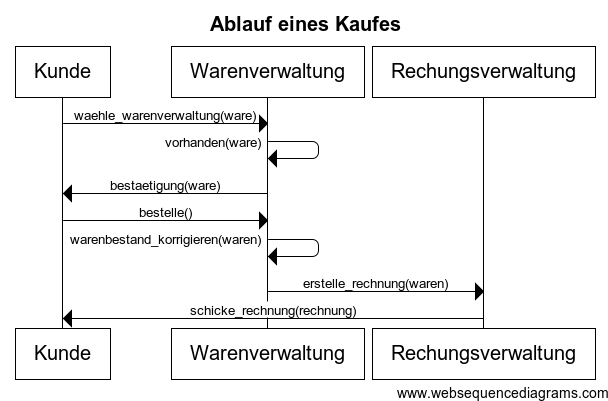
\includegraphics[scale=0.6]{kauf}
\end{figure}				
Auf Abbildung \ref{fig:kauf} nicht gezeigt, das entfernen der ausgew\"ahlten Waren. Hier wird der Ablauf des Bef\"ullen des Warenkorbs und der Ablauf der Bestellung gezeigt.

\subsection{Begr\"undung der gew\"ahlten Tenchnologien}
Zur Debate stand, welche Programmiersprache bzw. welche Scriptsprache, welchen Webserver und welches Datenbankmanagementsystem wir f\"ur die Entwicklung des Webshops verwenden. Zur Option stellten wir uns hier aufgrund der Bekanntheit Ruby on Rails und PHP.

\begin{figure}[h]
	\caption{Vergleich zwischen Rails und PHP}
	\cite{tbray}
	\label{fig:vergleich}
	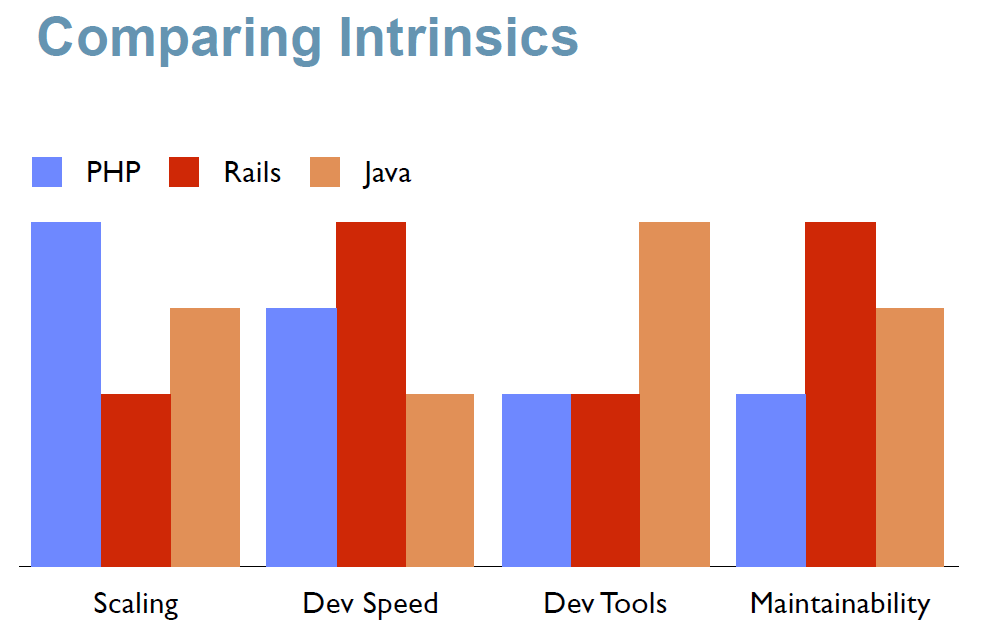
\includegraphics[scale=0.5]{complang}
\end{figure}

In Abbildung \ref{fig:vergleich} zu sehen, ist ein Vergleich zwischen Java, Ruby on Rails und PHP. Wir werden aufgrund der Entwicklungsgeschwindigkeit, der Wartbarkeit und dem Grund, dass wir Ruby in Programmieren I verwendeten, Ruby on Rails verwenden. Offen bleibt nun, welches Datenbankmanagementsystem und welchen Webserver wir verwenden. Wir sind uns derzeit beim DBMS uneinig ob wir MySQL oder SQLite verwenden.

\subsection{Design der Datenbank}

\subsection{Dokumentation}

\subsection{Offene Fragen}
\begin{itemize}
	\item MySQL oder SQLite?
\end{itemize}

\bibliographystyle{alpha}
\bibliography{./references}
\end{document}
